% !TEX encoding = UTF-8 Unicode
\documentclass[
10pt,
aspectratio=43,
]{beamer}
\setbeamercovered{transparent=10}
\usetheme[
%  showheader,
%  red,
  purple,
%  gray,
%  graytitle,
  colorblocks,
%  noframetitlerule,
]{Verona}

\usepackage[T1]{fontenc}
\usepackage{tikz}
\usepackage[utf8]{inputenc}
\usepackage{lipsum}
%%%%%%%%%%%%%%%%%%%%%%%%%%%%%%%
% Mac上使用如下命令声明隶书字体,windows也有相关方式,大家可自行修改
\providecommand{\lishu}{\CJKfamily{zhli}}
%%%%%%%%%%%%%%%%%%%%%%%%%%%%%%%
\usepackage{tikz}
\usetikzlibrary{fadings}
%
%\setbeamertemplate{sections/subsections in toc}[ball]
\usepackage{xeCJK}
\usepackage{listings}
\usepackage{caption}
\usepackage{subfigure}
\usefonttheme{professionalfonts}
\def\mathfamilydefault{\rmdefault}
\usepackage{amsmath}
\usepackage{multirow}
\usepackage{booktabs}
\usepackage{bm}
\setbeamertemplate{section in toc}{\hspace*{1em}\inserttocsectionnumber.~\inserttocsection\par}
\setbeamertemplate{subsection in toc}{\hspace*{2em}\inserttocsectionnumber.\inserttocsubsectionnumber.~\inserttocsubsection\par}
\setbeamerfont{subsection in toc}{size=\small}
\AtBeginSection[]{%
	\begin{frame}%
		\frametitle{Outline}%
		\textbf{\tableofcontents[currentsection]} %
	\end{frame}%
}

\AtBeginSubsection[]{%
	\begin{frame}%
		\frametitle{Outline}%
		\textbf{\tableofcontents[currentsection, currentsubsection]} %
	\end{frame}%
}

\title{高等数学C}
%\subtitle{A Simple while elegant template}
\author[P.Yu]{余沛}
\mail{peiy\_gzgs@qq.com}
\institute[Guangzhou College of Technology and Business]{Guangzhou College of Technology and Business \\
  广州工商学院}
\date{\today}
\titlegraphic[width=4cm]{logo.png}{}




%%%%%%%%%%%%%%%%%%%%%%%%%%%%%%%%
% ----------- 标题页 ------------
%%%%%%%%%%%%%%%%%%%%%%%%%%%%%%%%



\begin{document}

\maketitle

%%% define code
\defverbatim[colored]\lstI{
	\begin{lstlisting}[language=C++,basicstyle=\ttfamily,keywordstyle=\color{red}]
	int main() {
	// Define variables at the beginning
	// of the block, as in C:
	CStash intStash, stringStash;
	int i;
	char* cp;
	ifstream in;
	string line;
	[...]
	\end{lstlisting}
}
%%%%%%%%%%%%%%%%%%%%%%%%%%%%%%%%
% ----------- FRAME ------------
%%%%%%%%%%%%%%%%%%%%%%%%%%%%%%%%

\section{数列极限}
\subsection{回顾: 等价无穷小}
\begin{frame}
\begin{block}{无穷小量定义}设函数 $f(x)$ 在 $x=a$ 处有定义,如果对于任意给定的正数 $\varepsilon$,存在正数 $\delta$,使得当 $0 < |x-a| < \delta$ 时,有 $|f(x)| < \varepsilon$,则称函数 $f(x)$ 在 $x=a$ 处为无穷小量.
\end{block}
\begin{itemize}
\item<2-> \textbf{幂函数}: 当 $x$ 趋近于 $0$ 时,函数 $f(x) = x^n$ 是无穷小量,其中 $n$ 是正整数.\\
\item<3-> \textbf{指数函数}: 当 $x$ 趋近于 $0$ 时,函数 $f(x) = e^x - 1$ 是无穷小量.\\
\item<4-> \textbf{三角函数}: 当 $x$ 趋近于 $0$ 时,函数 $f(x) = \sin(x)$ 和 $f(x) = \tan(x)$ 是无穷小量.\\
\item<5-> \textbf{对数函数}: 当 $x$ 趋近于 $1$ 时,函数 $f(x) = \log(x)$ 是无穷小量.
\end{itemize}

\end{frame}
\begin{frame}
\frametitle{函数的无穷小量的比较}
当 $x\to0$ 时, $x, x^2, 2 x$ 都是无穷小量, 比较它们趋向于 0 的速度,
\begin{itemize}
\item $\lim _{x \rightarrow 0} \frac{x^2}{x}=0, x^2$ 比 $x$ 要快得多; 称 $x^2$ 是比 $x$ 高阶无穷小;
\item $\lim _{x \rightarrow 0} \frac{2 x}{x}=2,2 x$ 与 $x$ 大致相同; 称 $2 x$ 与 $x$ 是同阶无穷小;
\item $\lim _{x \rightarrow 0} \frac{x}{x^2}=\infty, x$ 比 $x^2$ 要慢得多.称 $x$ 是比 $x^2$ 较低阶无穷小.
\end{itemize}
\pause
\begin{block}{等价无穷小}
特别地,如果有
$$
\lim \frac{\alpha}{\beta} = 1,
$$
则称 $\beta$ 与 $\alpha$ 是等价无穷小量,记作 $\alpha ~ \beta$.
\end{block}
\end{frame}

\subsection{常用的等价无穷小}

\begin{frame}
\frametitle{等价无穷小替换定理与常用的等价无穷小}

\begin{block}{定理(无穷小等价替换定理)}
如果 $\alpha_{1 \hookleftarrow} \beta_1, \alpha_{2 \hookleftarrow} \beta_2$ 且极限 $\lim \frac{\beta_1}{\beta_2}$ 存在, 则
$$
\lim \frac{\alpha_1}{\alpha_2}=\lim \frac{\beta_1}{\beta_2}
$$
\end{block}
\pause
\begin{proof}
$\quad \lim \frac{\alpha_1}{\alpha_2}=\lim \frac{\alpha_1}{\beta_1} \cdot \frac{\beta_2}{\alpha_2} \cdot \frac{\beta_1}{\beta_2}=\lim \frac{\beta_1}{\beta_2}$.

\end{proof}
\pause
常用的等价无穷小:
当 $x \rightarrow 0$时
$$
 x \sim \sin x \sim \tan x \sim \arcsin x \sim \arctan x \sim \ln (x+1) \sim e^x-1,
$$
$$
1-\cos x \sim \frac{1}{2} x^2.
$$

\end{frame}

\begin{frame}
\frametitle{等价无穷小替换定理与常用的等价无穷小}
\begin{exampleblock}{例1}
 $ \quad \lim _{x \rightarrow 0} \frac{\tan m x}{\sin n x}=\lim _{x \rightarrow 0} \frac{m x}{n x}=\frac{m}{n} \quad(\tan m x \sim m x, \sin n x\sim n x)$
\end{exampleblock}
\pause
\begin{exampleblock}{例2}
 $ \lim _{x \rightarrow 0} \frac{\sin ^2 x}{x^3+2 x^2}=\lim _{x \rightarrow 0} \frac{x^2}{x^3+2 x^2}=\lim _{x \rightarrow 0} \frac{1}{x+2}=\frac{1}{2}\left(\sin ^2 x \sim x^2\right)$
\end{exampleblock}
\end{frame}
\begin{frame}
\frametitle{等价无穷小替换定理与常用的等价无穷小}
\begin{exampleblock}{例3}
\begin{equation*}
\begin{aligned}
&\lim _{x \rightarrow 1} \frac{\ln x}{x^2-1}=\lim _{x \rightarrow 1} \frac{\ln [1+(x-1)]}{(x+1)(x-1)}=\lim _{x \rightarrow 1} \frac{x-1}{(x+1)(x-1)}=\frac{1}{2},\\
&(\ln [(x-1)+1] \sim x-1)
\end{aligned}
\end{equation*}
\end{exampleblock}
\pause
\begin{exampleblock}{例4} \begin{equation*}
\begin{aligned}
& \lim _{x \rightarrow 0} \frac{\left(1+x^2\right)^{\frac{1}{3}}-1}{\cos x-1}=\lim _{x \rightarrow 0} \frac{\frac{1}{3} x^2}{-\frac{1}{2} x^2}= -\frac{2}{3}\\
& \left(\left(1+x^2\right)^{\frac{1}{3}}-1 \sim \frac{1}{3} x^2, \cos x-1 \sim-\frac{1}{2} x^2\right)
\end{aligned}
\end{equation*}
\end{exampleblock}
\end{frame}

\section{函数的连续性}
\subsection{增量与差分}

\begin{frame}
\frametitle{增量, 差分与函数连续性}
\begin{block}{增量}
\begin{itemize}
    \item $\Delta x: \Delta x=x_1-x_0$, 即自变量的增量 $=$ 终值 - 初值, 或终值 $x_1=x_0+\Delta x$;
    \item $\Delta y: \Delta y=y_1-y_0$, 即因变量的增量 $=$ 终值 - 初值, 或终值 $y_1=y_0+\Delta y$;
\end{itemize}
$\Delta x$, $\Delta y$ 也被称为关于自变量,因变量的差分.
\end{block}
\end{frame}

\begin{frame}
\frametitle{函数的连续性概念}
\begin{block}{函数的连续性}
 设函数 $y=f(x)$ 在点 $x_0$ 的某个邻域内有定义, 如果当自变量的增量 $\Delta x \rightarrow 0$ 时, 相应因变量的增量 $\Delta y \rightarrow 0$, 则称 $f(x)$ 在点 $x_0$ 处\textbf{连续},\\
 记作 $$\lim _{\Delta x \rightarrow 0} \Delta y=0$$. 
\end{block}
\pause
初等函数在定义域范围内都是连续的.
\pause
\begin{exampleblock}{不连续}
否则, 称 $f(x)$ 在点 $x_0$ 处不连续.
\end{exampleblock}
\pause
初等函数在不包含于定义域的区间上都是不连续的.

\begin{alertblock}{图像与极限存在}
	如果是能采用图像方法精确描述的函数,图像上没有跳点,断点或者无穷大趋势,那么在该点上函数是连续的.
\end{alertblock}

\end{frame}

\subsection{分段函数的连续性}
\begin{frame}
\frametitle{分段函数的连续性}
	可以通过研究左极限和右极限是否存在并相等的办法来研究.

\begin{block}{函数极限的数列定义}
	设函数 $f(x)$ 在点 $x=a$ 的某个去心邻域 $(a,b)/\{x\}$ 内有定义,如果存在常数 $L$,对于任意定义在该去心邻域上收敛到$a$的数列 $\{x_n\}$,都有 
 \begin{equation*}
\lim_{n\to\infty} f(x_n) = L,
 \end{equation*}
 则称函数 $f(x)$ 在 $x=a$ 处\textbf{收敛}于 $L$,记作 $\lim_{x \to a} f(x) = L$.
\end{block}
\begin{block}{定义: 左极限}
	设函数 $f(x)$ 在某个区间 $\bm{(a-\epsilon,a)}$ 内有定义,如果存在常数 $L$,对于任意定义在该区间上收敛到$a$的数列 $\{x_n\}$,都有 
 \begin{equation*}
\lim_{n\to\infty} f(x_n) = L,
 \end{equation*}
 则称函数 $f(x)$ 在 $x=a$ 处具有左极限 $L$,记作 $\lim_{x \to a^{-}} f(x) = L$.
\end{block}
\end{frame}

\begin{frame}{分段函数的连续性}
	同理,右极限应该这样定义: 
	\begin{block}{定义: 右极限}
			设函数 $f(x)$ 在某个区间 $\bm{(a,a+\epsilon)}$ 内有定义,如果存在常数 $L$,对于任意定义在该区间上收敛到$a$的数列 $\{x_n\}$,都有 
		\begin{equation*}
		\lim_{n\to\infty} f(x_n) = L,
		\end{equation*}
		则称函数 $f(x)$ 在 $x=a$ 处具有左极限 $L$,记作 $\lim_{x \to a^{+}} f(x) = L$.
	\end{block}
	\pause
	与函数的连续定义类似,我们可以模仿性地给出左连续,右连续的概念和与连续的概念.
	\begin{block}{定义: 左连续,右连续与连续}
		若 $\lim _{x \rightarrow x_0^{-}} f(x)=f\left(x_0\right)$,  则 $f(x)$ 在 $x_0$ 点左连续.\\
		若 $\lim _{x \rightarrow x_0^{+}} f(x)=f\left(x_0\right) $, 则 $f(x)$ 在 $x_0$ 点右连续.\\
		若 $\lim _{x \rightarrow x_0^{-}} f(x)=f\left(x_0\right)=\lim _{x \rightarrow x_0^{+}} f(x)$, 则称 $f(x)$ 在点 $x_0$ 处连续.
	\end{block}
\end{frame}

\begin{frame}{分段函数的连续性}
	有了左连续和右连续的概念,我们可以对分段函数间断点的连续性问题进行分析.
	\pause
	\begin{block}{间断点分类: 情况}
		\begin{equation*}
			\text{间断点}\left\{
				\begin{array}{ll}
					\text{左右极限都存在}\left\{
						\begin{array}{ll}
							\text{左右极限相等}\\
							\text{左右极限不相等}
						\end{array}
					\right.\\
					\text{左右极限至少一个不存在}
				\end{array}
			\right.
		\end{equation*}
	\end{block}
	\pause
	\begin{exampleblock}{间断点分类: 名称}
		\begin{equation*}
			\text{间断点}\left\{
				\begin{array}{ll}
					\text{第一类间断点}\left\{
						\begin{array}{ll}
							\text{可去间断点}\\
							\text{跳跃间断点(跃点)}
						\end{array}
					\right.\\
					\text{第二类间断点}
				\end{array}
			\right.
		\end{equation*}
	\end{exampleblock}
\end{frame}

\subsection{间断点概念}
\begin{frame}{分段函数的连续性}{可去间断点}
	\begin{columns}[onlytextwidth]
		\column{0.4\textwidth}
		\[
			f(x) = \begin{cases}
			\sin(x) & \text{if } x < 0 \\
			\sqrt{x} & \text{otherwise}
			\end{cases}
		\]
		\column{0.6\textwidth}
		\begin{tikzpicture}
			\draw[->] (-3.5,0) -- (3.5,0) node[right] {$x$};
			\draw[->] (0,-1.5) -- (0,1.5) node[above] {$y$};
			
			\draw[domain=-3:0,smooth,variable=\x,blue] plot ({\x},{sin(\x r)});
			\draw[domain=0:3,smooth,variable=\x,red] plot ({\x},{sqrt(\x)});
			
			\node[blue] at (-2,-1) {$y = \sin(x)$};
			\node[red] at (2,1) {$y = \sqrt{x}$};
		  \end{tikzpicture}
	\end{columns}
\end{frame}

\begin{frame}{分段函数的连续性}{跳跃间断点}
	\begin{columns}[onlytextwidth]
		\column{0.4\textwidth}
		\[
			f(x) = \begin{cases}
			-1 & \text{if } x < 0 \\
			0 & \text{if } x = 0 \\
			1 & \text{if } x > 0
			\end{cases}
			\]
		\column{0.6\textwidth}
		\begin{tikzpicture}
			\draw[->] (-3.5,0) -- (3.5,0) node[right] {$x$};
			\draw[->] (0,-1.5) -- (0,1.5) node[above] {$y$};
			
			\draw[domain=-3:0,smooth,variable=\x,blue] plot ({\x},{-1});
			\draw[domain=0:3,smooth,variable=\x,red] plot ({\x},{1});
			
			\node[blue] at (-2,-1) {$y = -1$};
			\node[red] at (2,1) {$y = 1$};
			
			\draw (-0.1,-1) -- (0.1,-1) node[right] {$-1$};
			\draw (-0.1,1) -- (0.1,1) node[right] {$1$};
			\draw (3,-0.1) -- (3,0.1) node[above] {$3$};
		  \end{tikzpicture}
	\end{columns}
\end{frame}

\begin{frame}{分段函数的连续性}{第二类间断点}
	\begin{columns}[onlytextwidth]
		\column{0.4\textwidth}
		\[
			f(x) = e^{\frac{1}{|x|-1}}
			\]
		\column{0.6\textwidth}
		\begin{figure}
			\centering
			% Requires \usepackage{graphicx}
			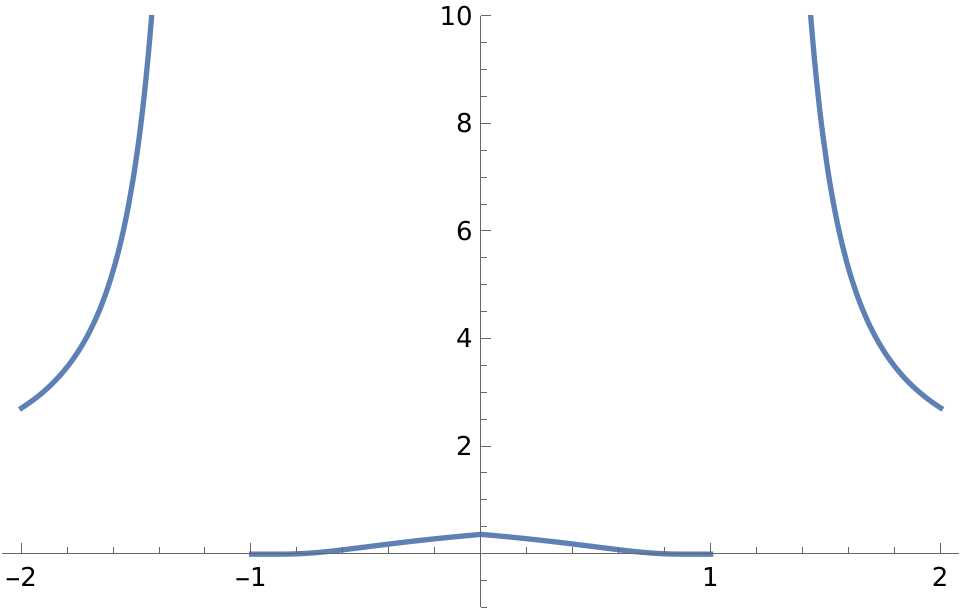
\includegraphics[width=5cm]{Exp[1/(Abs[x]-1)}
		\end{figure}
	\end{columns}
\end{frame}

\begin{frame}{分段函数的连续性}{判断间断点}
\begin{exampleblock}{Dirichlet 函数 $D(x)$}
	\[
		D(x) = \begin{cases}
		1 & \text{if } x \in \mathbb{Q}, \\
		0 & \text{if } x \in \mathbb{R} \setminus \mathbb{Q}.
		\end{cases}
		\]

\end{exampleblock}
\pause
\begin{exampleblock}{Riemann 函数 $R(x)$}
	\[
		R(x) = \begin{cases}
			\displaystyle\frac1q & \text{if } x = \displaystyle\frac{p}{q}\in \mathbb{Q},\,\,gcd(p,q)=1, \\
		0 & \text{if } x \in \mathbb{R} \setminus \mathbb{Q}.
		\end{cases}
		\]

\end{exampleblock}

\end{frame}


	


\subsection{连续函数的性质}

\begin{frame}{连续函数的性质}{连续性判定}
	\begin{exampleblock}{四则运算性质}
		若函数 $f(x), g(x)$ 在 $x_0$ 处连续, 则它们的和、差、积、商(分 母不为 0 ) 在 $x_0$ 处也连续.
	\end{exampleblock}
	\pause
	\begin{exampleblock}{复合运算性质}
		若函数 $u=\varphi(x)$ 在 $x_0$ 处连续, 而函数 $y=f(u)$ 在 $u_0=\varphi\left(x_0\right)$ 处也连续, 则复合函数 $y=f(\varphi(x))$ 在 $x=x_0$ 处连 续, 即有 $\lim _{x \rightarrow x_0} f[\varphi(x)]=f\left[\varphi\left(x_0\right)\right]$
	
	\end{exampleblock}
	\pause
	\begin{exampleblock}{反函数的连续性}
		单调递增 (递减) 且连续的函数, 其反函数也单调递增 (递减) 且连续.
	\end{exampleblock}
	
\end{frame}

\begin{frame}{连续函数的性质}{初等函数的连续性}
	\begin{block}{基本初等函数的连续性}
		$x^n (x>0,n>1)$, $\sin(x)$, $e^x$ 是连续的.
	\end{block}
	Why?
	\pause
	\begin{exampleblock}{反函数连续性扩张定义}
		$x^n (x>0,n>0)$, $\arcsin(x)$, $\log{x}$, 在其定义域上是连续的.
	\end{exampleblock}
	\pause
	\begin{exampleblock}{加点四则运算和复合运算}
		\[\left(\frac{\lg (100+x)}{4^x+\arcsin x}\right)^{\frac{1}{2}},\]

		\[-\frac{1}{4} \sqrt{\tan \frac{e^{\arccos x}}{2}} \cdot \csc ^2 \frac{\log x}{2}.\]
	\end{exampleblock}
	
\end{frame}

\subsection{闭区间上连续函数的性质}
\begin{frame}{连续函数的性质}{连续函数在区间上的连续性}
	\begin{block}{基本初等函数的连续性}
		开区间连续: 若 $f(x)$ 在 $(a, b)$ 中每一点都连续, 则称 $f(x)$ 在 $(a, b)$ 连续.\pause \\
		闭区间连续: 若 $f(x)$ 在 $(a, b)$ 中每一点都连续, 在 $a$ 点右连续, 在 $b$ 点左连续, 则称 $f(x)$ 在 $[a, b]$ 连续.
	\end{block}
	\pause 有什么区别呢?\pause {\bf 函数在端点上的连续性.}
\end{frame}

\begin{frame}{连续函数的性质}{连续函数在闭区间上的连续性}
	\begin{block}{定义: 最大值和最小值}
		设函数 $y=f(x)$ 在区间 $I$ 上有定义, 如果存在 $x_1, x_2 \in I$, 使得对任意的 $x \in I$, 有
		$$
		f\left(x_2\right) \leq f(x) \leq f\left(x_1\right),
		$$
		则称 $f\left(x_1\right), f\left(x_2\right)$ 分别为函数 $y=f(x)$ 在 $I$ 上的最大值和最小值, 点 $x_1, x_2$ 叫做 $y=f(x)$ 的最大值点和最小值点.
	\end{block}
	\pause
	\begin{block}{最值定理}
		若函数 $y=f(x)$ 在 $[a, b]$ 上连续, 则 $y=f(x)$ 在 $[a, b]$ 上必 取得最大值和最小值.
	\end{block}
	\pause 与 $I$ 的开闭性的关联?\pause {\bf 函数端点的连续性.}\pause 
	\begin{equation*}
		f(x) = x^{-1},\quad x\in(0,1).
	\end{equation*}
	\pause 以及推论: 闭区间上的连续函数是有界的.\\
	\pause (开区间,半开半闭区间则没有这个结论)
\end{frame}

\begin{frame}{连续函数的性质}{连续函数在闭区间上的连续性}
	\begin{block}{介值定理}
		设 $y=f(x)$ 在 $[a, b]$ 上连续, $M$ 和 $m$ 为 $y=f(x)$ 在 $[a, b]$ 上的最大值和最小值, 则任给值 $c$ : $m<c<M$, 存在 $\xi \in(a, b)$, 使得 $f(\xi)=c$.
	\end{block}
	\pause 如何证明? \pause 二分逼近与二分求解.
	\begin{block}{推论}
		若函数 $y=f(x)$ 在 $[a, b]$ 上连续, 且 $f(a) f(b)<0$, 则存在 $\xi \in(a, b)$, 使得
		$$
		f(\xi)=0 .
		$$
	\end{block}

	\begin{exampleblock}{例题}
		证明方程 $x^5-3 x=1$ 至少有一个根介于 1 和 2 之间.
	\end{exampleblock}
	\begin{equation*}
		f(x):x^5-3 x-1, \,\, \pause f(1)=-3, \,\, \pause f(2)=32-6-1=25,\,\, \pause f(1)\cdot f(2) =-75.
	\end{equation*}
\end{frame}

\subsubsection{有界性}
\subsubsection{介值性与零点存在定理}




% Thank you page
\beamertemplateshadingbackground{structure.fg!90}{structure.fg}
\begin{frame}[plain]
	\vfill
	\centering
	{
		\centering \Huge \color{white} Thank you for your attention!\\[10pt]Questions?\bigskip \\
		Homework: Page 82: 28, 31, 36.
	}
	\vfill
\end{frame}


\end{document}


